\documentclass[border=8pt]{standalone}
\usepackage[T1]{fontenc}\usepackage[utf8]{inputenc}
\usepackage{helvet}\renewcommand{\familydefault}{\sfdefault}
\usepackage{tikz,xcolor}
\usetikzlibrary{arrows.meta,positioning,shapes.geometric,shapes.multipart,calc,fit,backgrounds,decorations.markings}
\definecolor{ink}{HTML}{1E1B16}\definecolor{paper}{HTML}{FBF8F2}\definecolor{clay}{HTML}{B5482A}\definecolor{soft}{HTML}{F1E9DA}\definecolor{pine}{HTML}{24402F}
\tikzset{
  every node/.style={font=\small,text=ink},
  >=Stealth, line/.style={draw=ink,line width=0.8pt},
  cls/.style={rectangle split,rectangle split parts=3,draw=ink,line width=0.8pt,fill=soft,align=left,inner xsep=6pt,inner ysep=4pt,
              rectangle split part align={center,left,left},minimum width=3.0cm},
  cls2/.style={rectangle split,rectangle split parts=2,draw=ink,line width=0.8pt,fill=soft,align=left,inner xsep=6pt,inner ysep=4pt,
              rectangle split part align={center,left},minimum width=3.0cm},
  box/.style={rectangle,draw=ink,line width=0.8pt,fill=soft,align=center,inner sep=5pt,minimum height=0.8cm},
  state/.style={rectangle,rounded corners=8pt,draw=ink,line width=0.8pt,fill=soft,align=center,inner sep=6pt,minimum width=2.2cm,minimum height=0.9cm},
  act/.style={rectangle,rounded corners=10pt,draw=ink,line width=0.8pt,fill=soft,align=center,inner sep=5pt,minimum width=2.4cm,minimum height=0.8cm},
  dec/.style={diamond,draw=ink,line width=0.8pt,fill=soft,inner sep=1pt,minimum width=0.9cm,minimum height=0.9cm},
  uc/.style={ellipse,draw=ink,line width=0.8pt,fill=soft,align=center,inner sep=3pt,minimum width=3.2cm,minimum height=1.0cm},
  note/.style={rectangle,draw=ink,line width=0.6pt,fill=yellow!12,align=left,inner sep=4pt,font=\footnotesize},
  lab/.style={font=\footnotesize,fill=paper,inner sep=1.5pt},
  err/.style={},
}
\newcommand{\actor}[3]{% x,y,label
  \draw[line width=0.8pt] (#1,#2+0.55) circle (0.17);
  \draw[line width=0.8pt] (#1,#2+0.38)--(#1,#2-0.15) (#1-0.3,#2+0.22)--(#1+0.3,#2+0.22) (#1,#2-0.15)--(#1-0.25,#2-0.6) (#1,#2-0.15)--(#1+0.25,#2-0.6);
  \node[font=\small] at (#1,#2-0.9) {#3};}
\begin{document}
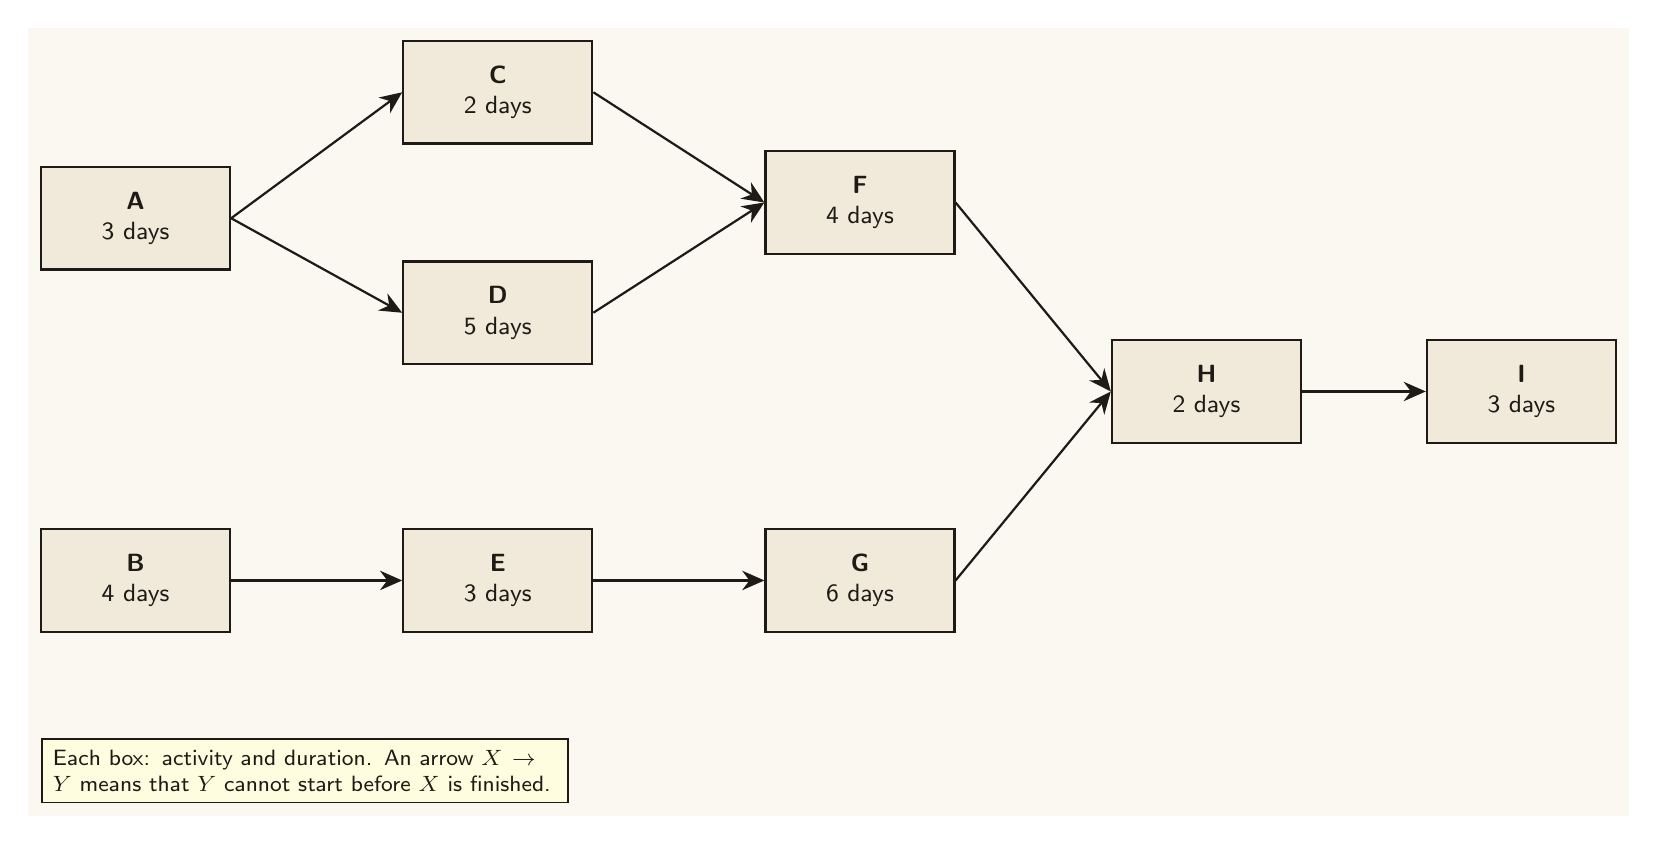
\begin{tikzpicture}[background rectangle/.style={fill=paper},show background rectangle]
\node[box,minimum width=2.4cm,minimum height=1.3cm] (A) at (0,2.6) {\textbf{A}\\ 3 days};
\node[box,minimum width=2.4cm,minimum height=1.3cm] (B) at (0,-2.0) {\textbf{B}\\ 4 days};
\node[box,minimum width=2.4cm,minimum height=1.3cm] (C) at (4.6,4.2) {\textbf{C}\\ 2 days};
\node[box,minimum width=2.4cm,minimum height=1.3cm] (D) at (4.6,1.4) {\textbf{D}\\ 5 days};
\node[box,minimum width=2.4cm,minimum height=1.3cm] (E) at (4.6,-2.0) {\textbf{E}\\ 3 days};
\node[box,minimum width=2.4cm,minimum height=1.3cm] (F) at (9.2,2.8) {\textbf{F}\\ 4 days};
\node[box,minimum width=2.4cm,minimum height=1.3cm] (G) at (9.2,-2.0) {\textbf{G}\\ 6 days};
\node[box,minimum width=2.4cm,minimum height=1.3cm] (H) at (13.6,0.4) {\textbf{H}\\ 2 days};
\node[box,minimum width=2.4cm,minimum height=1.3cm] (I) at (17.6,0.4) {\textbf{I}\\ 3 days};
\draw[line,-{Stealth[length=8pt,width=7pt]}] (A.east)--(C.west);
\draw[line,-{Stealth[length=8pt,width=7pt]}] (A.east)--(D.west);
\draw[line,-{Stealth[length=8pt,width=7pt]}] (B.east)--(E.west);
\draw[line,-{Stealth[length=8pt,width=7pt]}] (C.east)--(F.west);
\draw[line,-{Stealth[length=8pt,width=7pt]}] (D.east)--(F.west);
\draw[line,-{Stealth[length=8pt,width=7pt]}] (E.east)--(G.west);
\draw[line,-{Stealth[length=8pt,width=7pt]}] (F.east)--(H.west);
\draw[line,-{Stealth[length=8pt,width=7pt]}] (G.east)--(H.west);
\draw[line,-{Stealth[length=8pt,width=7pt]}] (H.east)--(I.west);
\node[note,anchor=north west,text width=6.4cm] at (-1.2,-4.0) {Each box: activity and duration. An arrow $X \rightarrow Y$ means that $Y$ cannot start before $X$ is finished.};
\end{tikzpicture}
\end{document}
